\documentclass[ngerman,a4paper,order=firstname]{../../texmf/tex/latex/mathscript/mathscript}
\usepackage{../../texmf/tex/latex/mathoperators/mathoperators}

\title{\textbf{Stochastik SS 2019}}
\author{Dozent: Prof. Dr. \person{Anita Behme}}

% local commands
\renewcommand{\F}{\mathscr F}
%\undef{\P}
\renewcommand{\P}{\mathbb{P}}
%\undef{\O}
\renewcommand{\O}{\Omega}
%\undef{\G}
\renewcommand{\G}{\mathscr{G}}
%\undef{\base}
\newcommand{\E}{\mathcal{E}}

\def\upmodels{\perp\!\!\!\perp}

\begin{document}
\pagenumbering{roman}
\pagestyle{plain}

\maketitle

\hypertarget{tocpage}{}
\tableofcontents
\bookmark[dest=tocpage,level=1]{Inhaltsverzeichnis}

\pagebreak
\pagenumbering{arabic}
\pagestyle{fancy}

\chapter*{Vorwort}
Schön, dass du unser Skript für die Vorlesung \textit{Lineare Algebra und analytische Geometrie 1} bei Prof. Dr. Arno Fehm im WS2017/18 gefunden hast! \footnote{Obwohl man sagen kann, dass es in dieser Vorlesung nur um Lineare Algebra ging, der Teil mit der analytischen Geometrie wurde vernachlässigt. Liegt wahrscheinlich auch daran, dass es demnächst eine Reform der Studienordnung gibt, in der aus der Vorlesung \textit{Lineare Algebra und analytische Geometrie} die Vorlesung \textit{Einführung in die Lineare Algebra} wird.}

Wir verwalten dieses Skript mittels Github \footnote{Github ist eine Seite, mit der man Quelltext online verwalten kann. Dies ist dahingehend ganz nützlich, dass man die Quelltext-Dateien relativ einfach miteinander synchronisieren kann, wenn man mit mehren Leuten an einem Projekt arbeitet.}, d.h. du findest den gesamten \LaTeX-Quelltext auf \url{https://github.com/henrydatei/TUD_MATH_BA}. Unser Ziel ist, für alle Pflichtveranstaltungen von \textit{Mathematik-Bachelor} ein gut lesbares Skript anzubieten. Für die Programme, die in den Übungen zur Vorlesung \textit{Programmieren für Mathematiker} geschrieben werden sollen, habe ich ein eigenes Repository eingerichtet; es findet sich bei \url{https://github.com/henrydatei/TU_PROG}.

Du kannst dir gerne dort die \LaTeX-Quelldateien herunterladen, die Dateien für exakt dieses Skript sind im Ordner \texttt{1. Semester/LAAG ueberarbeitet}. Es lohnt sich auf jeden Fall während des Studiums die Skriptsprache \LaTeX{} zu lernen, denn Dokumente, die viele mathematische oder physikalische Formeln enthalten, lassen sich sehr gut mittels \LaTeX{} darstellen, in Word oder anderen Office-Programmen sieht so etwas dann eher dürftig aus.

\LaTeX{} zu lernen ist gar nicht so schwierig, ich habe dafür am Anfang des ersten Semesters wenige Wochen benötigt, dann kannte ich die wichtigsten Befehle und konnte den Vorgänger dieses Skriptes schreiben (\texttt{1. Semester/LAAG}, Vorsicht: hässlich, aber der Quelltext ist relativ gut verständlich).

Es sei an dieser Stelle darauf hingewiesen (wie in jedem anderem Skript auch \smiley{}), dass dieses Skript nicht den Besuch der Vorlesungen ersetzen kann. Es könnte sein, dass Prof. Fehm seine Vorlesung immer mal wieder an die Studenten anpasst; wahrscheinlich immer dann, wenn die Prüfungsergebnisse zu schlecht waren. Nichtsdestotrotz veröffentlicht Prof. Fehm sein Skript auf seiner Homepage \url{http://www.math.tu-dresden.de/~afehm/lehre.html}. Allerdings ist dieses Skript recht hässlich, besonders was die Übersichtlichkeit angeht.

Wir möchten deswegen ein Skript bereitstellen, dass zum einen übersichtlich ist, zum anderen \textit{alle} Inhalt aus der Vorlesung enthält, das sind insbesondere Diagramme, die sich nicht im offiziellen Skript befinden, aber das Verständnis des Inhalts deutlich erleichtern. Ich denke, dass uns dies erfolgreich gelungen ist.

Trotz intensivem Korrekturlesen können sich immer noch Fehler in diesem Skript befinden. Es wäre deswegen ganz toll von dir, wenn du auf unserer Github-Seite \url{https://github.com/henrydatei/TUD_MATH_BA} ein neues Issue erstellst und damit auch anderen hilfst, dass dieses Skript immer besser wird.

\chapter*{Was ist Stochastik?}

Altgriechisch Stochastikos ($\sigma \tau o \chi \alpha \sigma \tau \iota \kappa$\`{o}$ \zeta$) und bedeutet sinngemäß ``scharfsinning in Vermuten''.\\
Fragestellung insbesondere aus Glückspiel, Versicherung-/Finanzmathematik, überall da wo Zufall/ Risiko / Chance auftauchen.\\
Was ist Stochastik?
\begin{itemize}
	\item Beschreibt zufällige Phänomene in einer exakten Spache!\\
	Beispiel: ``Beim Würfeln erscheint jedes sechste Mal (im Schnitt) eine 6.'' $\longrightarrow$ Gesetz der großen Zahlen ($\nearrow$ später) %TODO set ref
	\item Lässt sich mathematische Stochastik in zwei Teilgebiete unterteilen\\
	Wahrscheinlichkeitstheorie (W-Theorie) \& Statistik
	\begin{itemize}
		\item \textit{W-Theorie}: Beschreibt und untersucht konkret gegebene Zufallssituationen.
		\item \textit{Statistik}: Zieht Schlussfolgerungen aus Beobachtungen.
	\end{itemize}
	Statistik benötigt Modelle der W-Theorie und W-Theorie benötigt die Bestätigung der Modelle durch Statistik.
\end{itemize}
In diesem Semester konzentrieren wir uns nur auf die Wahrscheinlichkeitstheorie!
% Grundbegriffe der WTheorie
\chapter{Grundbegriffe der Wahrscheinlichkeitstheorie}

\section{Wahrscheinlichkeitsräume}

\subsection*{Ergebnisraum}

Welche der möglichen Ausgänge eines zufälligen Geschehens interessieren uns?\\
Würfeln? Augenzahl, nicht die Lage und die Fallhöhe

\begin{definition}[Ergebnisraum]
	Die Menge der relevanten Ergebnisse eines Zufallsgeschehens nennen wir \begriff{Ergebnisraum} und bezeichnen diesen mit $\Omega$.
\end{definition}

\begin{*example}
	\begin{itemize}
		\item Würfeln: $\Omega = \{1,2, \dots, 6\}$
		\item Wartezeiten: $\Omega = \real_{+} = [0, \infty)$ (überabzählbar!)
	\end{itemize}
\end{*example}

\subsection*{Ereignisse}

Oft interessieren wir uns gar nicht für das konkrete Ergenis des Zufallsexperiments, sondern nur für das Eintreten gewisser Ereignisse.
\begin{*example}
	\begin{itemize}
		\item Würfeln: Zahl ist $\ge 3$
		\item Wartezeit: Wartezeit $\le 5$ Minuten
	\end{itemize}
\end{*example}

$\longrightarrow$ Teilmenge des Ereignisraums, also Element der Potenzmenge $\mathscr{P}(\Omega)$, denen eine Wahrscheinlichkeit zugeordnet werden kann, d.h. welche \begriff{messbar} (mb) sind.

\begin{definition}[Ereignisraum, messbarer Raum]
	Sei $\Omega \neq \emptyset$ ein Ergebnisraum und $\mathscr{F}$ eine $\sigma$-Algebra auf $\Omega$, d.h. eine Familie von Teilmenge von $\Omega$, sodass
	\begin{enumerate}
		\item $\Omega \in \mathscr{F}$
		\item $A \in \mathscr{F} \Rightarrow A^C \in \mathscr{F}$
		\item $A_1, A_2, \dots \in \mathscr{F} \Rightarrow \bigcup_{i \ge 1} \in \mathscr{F}$
	\end{enumerate}
	Dann heißt $(\Omega, \mathscr{F})$ \begriff{Ereignisraum} bzw. \begriff{messbarer Raum}.
\end{definition}

\subsection*{Wahrscheinlichkeiten}

Ordne Ereignissen Wahrscheinlichkeiten zu mittels der Abbildung

\begin{align}
	\mathbb{P}: \mathscr{F} \to [0,1]\notag
\end{align}

sodass

\begin{align}
	\text{Normierung } \mathbb{P}(\Omega) = 1 \tag{N}\label{eq_norm}\\
	\sigma\text{-Additivität für paarweise disjunkte Ereignisse} \tag{A}\label{eq_additive}\\
	A_1, A_2, \dots \in \mathscr{F} \Rightarrow \mathbb{P}(\bigcup_{i \ge 1} A_i) = \sum_{1 \ge 1} \mathbb{P}(A_i)\notag
\end{align}

(\ref{eq_norm}), (\ref{eq_additive}) und die Nichtnegativität von $\mathbb{P}$ werden als \begriff{\person{Kolmogorov}sche Axiome} bezeichnet (nach Kolomogorov: Grundbegriffe der Wahrscheinlichkeitstheorie, 1933)

\begin{definition}[Wahrscheinlichkeitsmaß, Wahrscheinlichkeitsverteilung]
	Sei $(\Omega, \mathscr{F})$ ein Ereignisraum und $\mathbb{P}: \mathscr{F} \to [0,1]$ eine Abbildung mit Eigenschaften (\ref{eq_norm}) und (\ref{eq_additive}). Dann heißt $\mathbb{P}$ \begriff{Wahrscheinlichkeitsmaß} oder auch \begriff{Wahrscheinlichkeitsverteilung}.
\end{definition}

Aus der Definition folgen direkt:

\begin{proposition}[Rechenregeln für W-Maße]
	Sei $\mathbb{P}$ ein W-Maß, Ereignisse $(\Omega, \mathscr{F}), A, B, A_1, A_2, \dots \in \mathscr{F}$. Dann gelten:
	\begin{enumerate}
		\item $\mathbb{P}(\emptyset) = 0$
		\item Monotonie: $A \subseteq B \Rightarrow \mathbb{P}(A) \le \mathbb{P}(B)$
		\item endliche $\sigma$-Additivität: $\mathbb{P}(A\cup B) + \mathbb{P}(A\cap B) = \mathbb{P}(A) + \mathbb{P}(B)$ und insbesondere $\mathbb{P}(A) + \mathbb{P}(A^C) = 1$
		\item $\sigma$-Subadditivität:
		\begin{align}
			\mathbb{P}\left(\bigcup_{i \ge 1} A_i\right) \le \sum_{1 \ge 1} \mathbb{P}(A_i)\notag
		\end{align}
		\item $\sigma$-Stetigkeit: Wenn $A_n \uparrow A$ (d.h. $A_1 \subseteq A_2 \subseteq \cdots$ und $A = \bigcup_{i=1}^{\infty} (A_i)$) oder $A_n \downarrow A$, so gilt:
		\begin{align}
			\mathbb{P}(A_n) \longrightarrow \mathbb{P}(A), n \to \infty \notag
		\end{align}
	\end{enumerate}
\end{proposition}

\begin{proof}
	In der Vorlesung wurde nur auf Schillings MINT Vorlesung verwiesen. Der folgende Beweis wurde ergänzt.\\
	Beweise erst folgende Aussage: $A\cap B = \emptyset \Longrightarrow \probp(A \uplus B) = \probp(A) + \probp(B)$.\\
	Es kann $\sigma$-Additivität verwendet werden, indem ``fehlende'' Mengen durch $\emptyset$ ergänzt werden:
	\begin{align}
		\probp(A \uplus B) = \probp(A \uplus B \uplus \emptyset \uplus \emptyset \dots) = \probp(A) + \probp(B) + \probp(\emptyset) + \dots = \probp(A) + \probp(B),\notag
	\end{align}
	wobei Maßeigenschaften verwendet wurden.
	\begin{enumerate}
		\item Definition des Maßes.
		\item Da $A \subseteq B$ ist auch $B = A \uplus (B \setminus A) = A \uplus (B \setminus (A \cap B))$. Wende wieder Aussage von oben an, damit folgt
		\begin{align}
			\probp(B) = \probp(A \uplus (B \setminus A)) = \probp(A) + \probp(B \setminus A) \ge \probp(A) \label{eq_1_1_4}\tag{*}
		\end{align}
		\item Zerlege $A \cup B$ geschickt, dann sieht man mit oben gezeigter Aussage und (\ref{eq_1_1_4})
		\begin{align}
			\probp(A \cup B) + \probp(A \cap B) &= \probp(A \uplus (B \setminus (A \cap B)) + \probp(A \cap B)\notag \\
			&= \probp(A) + \probp(B \setminus (A \cap B)) + \probp(A \cap B)\notag\\
			&= \probp(A)+\probp(B).\notag	
		\end{align}
		Im letzten Schritt wurde (\ref{eq_1_1_4}) verwendet.
		\item Folgt aus endlicher $\sigma$-Additivität, da $\probp\left(\bigcap_{i\ge 1} A_i \right) \ge 0$.
		\item Definiere $F_1 := A_1, F_2 := A_2 \setminus A_1, \dots, F_{i+1} := A_{i+1}\setminus A_n$. Die $F_i$ Mengen sind paarweise disjunkt und damit folgt für $m \to \infty$
		\begin{align}
			A_m = \biguplus_{i=1}^{m} F_i \Rightarrow A = \biguplus_{i=1}^{\infty} F_i = \biguplus_{i=1}^{\infty} A_i\notag
		\end{align}
		und
		\begin{align}
			\probp(A) = \probp\left( \biguplus_{i=1}^{\infty} F_i \right) = \sum_{i=1}^{\infty} \probp(F_i) = \lim\limits_{m \to \infty} \probp\left( \biguplus_{i=1}^{m} F_i \right) = \lim\limits_{m\to \infty} \probp(A_m). \notag
		\end{align}
	\end{enumerate}
\end{proof}

\begin{example}
	Für ein beliebigen Ereignisraum $(\Omega, \mathscr{F})$ ($\Omega \neq \emptyset$) und eine beliebiges Element $\xi \in \Omega$ definiere
	\begin{align}
		\delta_{\xi}(A := \begin{cases}
		1 & \xi \in A \\
		0 & \text{ sonst}
		\end{cases}\notag
	\end{align}
	eine (degeneriertes) W-Maß auf $(\Omega, \mathscr{F})$, welches wir als \begriff{\person{Dirac}-Maß} oder \begriff{\person{Dirac}-Verteilung} bezeichnen.
\end{example}

\begin{example}
	Würfeln mit fairem, $6$-(gleich)seitigem Würfel mit Ergebnismenge $\Omega=\{1, \dots, 6\}$ und Ereignisraum $\mathscr{F} = \mathscr{P}(\Omega)$ setzen wir als Symmetriegründen
	\begin{align}
		\mathbb{P}(A) = \frac{\# A}{6}.\notag
	\end{align}
	(Wobei $\# A$ oder auch $\vert A \vert$ die Kardinalität von $A$ ist.) Das definiert ein W-Maß.
\end{example}

\begin{example}
	\proplbl{1_1_7}
	Wartezeit an der Bushaltestelle mit Ergebnisraum $\Omega = \real_{+}$ und Ereignisraum \person{Borel}sche $\sigma$-Algebra $\mathscr{B}(\real_{+}) = \mathscr{F}$. Eine mögliches W-Maß können wir dann durch
	\begin{align}
	\mathbb{P}(A) = \int_{A} \lambda e^{-\lambda x} \diff x\notag %TODO set a mathoperator for dx!!!
	\end{align}
	für einen Parameter $\lambda > 0$ festlegen. (Offenbar gilt $\mathbb{P}(\Omega) = 1$ und die $\sigma$-Additivität aufgrund der Additivität des Integrals.) Wir bezeichnen diese Maß als \begriff{Exponentialverteilung}. (Warum gerade dieses Maß für Wartezeiten gut geeignet ist $\nearrow$ später) %TODO add later a ref!!!
\end{example}

%%%%%%%%%%%%%%%%%%%%%%%%%%%%%%%% 2nd Lecture %%%%%%%%%%%%%%%%%%%%%%%%%%%%%%%%%%%%%%%%%%%%

\begin{proposition}[Konstruktion von WMaßen durch Dichten]
	Sei $(\Omega, \mathscr{F})$ ein Eriegnisraum.
	\begin{itemize}
		\item $\Omega$ abzählbar, $\mathscr{F} = \mathscr{P}(\Omega)$: Sei $\rho = (\rho(\omega))_{\omega \in \Omega}$ eine Folge in $[0,1]$ in $\sum_{\omega \in \Omega} \rho(\omega) = 1$, dann definiert
		\begin{align}
			\probp(A) = \sum_{\omega \in \Omega} \rho(\omega), A \in \mathscr{F} \notag
		\end{align}
		ein (diskretes) WMaß $\probp$ auf $(\Omega, \mathscr{F})$. $\rho$ wird als \begriff{Zähldichte} bezeichnet.
		\item Umgekehrt definiert jedes WMaß $\probp$ auf $(\Omega, \mathscr{F})$ definiert Folge $\rho(\omega) = \probp(\set{\omega}), \omega \in \Omega$ eine Folge $\rho$ mit den obigen Eigenschaften.
		\item $\Omega \subset \Rn, \mathscr{F} = \mathscr{B}(\Omega)$: Sei $\rho: \Omega \to [0, \infty)$ eine Funktion, sodass
		\begin{enumerate}
			\item $\int_{\Omega} \rho(x)\diff x = 1$
			\item $\set{x \in \Omega \colon f(x) \le c} \in \mathscr{B}(\Omega)$ für alle $c > 0$ 
		\end{enumerate}
		dann definiert $\rho$ ein WMaß $\probp$ auf $(\Omega, \mathscr{F})$ durch 
		\begin{align}
		\probp(A) = \int_{A} \rho(x) \diff x = \int_{A} \rho \diff \lambda, \quad A \in \mathscr{B}(\Omega).
		\end{align}
		Das Integral interpretieren wir stets als Lebesgue-Integral bzw. Lebesgue-Maß $\lambda$.
		$\rho$ bezeichnet wir als \begriff{Dichte}, \begriff{Dichtefunktion}/\begriff{Wahrscheinlichkeitsdichte} von $\probp$ und nennen ein solches $\probp$ \begriff{(absolut)stetig (bzgl. denn Lebesgue-Maß)}.
	\end{itemize}
\end{proposition}

\begin{proof}
	\begin{itemize}
		\item Der diskrete Fall ist klar.
		\item Im stetigen Fall folgt die Bahuptung aus den bekannten Eigenschaften des Lebesgue-Integrals ($\nearrow$ Schilling MINT, Lemma 8.9)
	\end{itemize}
\end{proof}

\begin{*remark}
	\begin{itemize}
		\item Die Eineindeutige Beziehung zwischen Dichte und WMaß überträgt sich nicht auf den stetigen Fall.
		\begin{itemize}
			\item Nicht jedes WMaß auf $(\Omega, \mathscr{B}(\Omega)), \Omega \subset \Rn$ besitzt eine Dichte.
			\item Zwei Dichtefunktionen definieren dasselbe WMaß, wenn sie sich nur auf einer Menge von Lebesgue-Maß $0$ unterscheiden.
		\end{itemize}
		\item Jede auf $\Omega \subset \Rn$ definiert Dichtefunktion $\rho$ lässt sich auf ganz $\Rn$ fortsetzen durch $\rho(x) = 0, x \not\in \Omega$. Das erzeugte WMaß auf $(\Rn, \mathscr{B}(\Omega))$ lässt mit den WMaß auf $(\Omega, \mathscr{\Omega})$ identifizieren.
		\item Mittels Dirac-Maß $\delta_{x}$ können auch jedes diskrete WMaß auf $\Omega \subset \Rn$ als WMaß auf $\Rn, \mathscr{B}(\Rn)$ intepretieren
		\begin{align}
			\probp(A) = \sum_{\omega \in A} \rho(\omega) = \int_{A} \diff \left( \sum_{\omega \in \Omega} \rho(\omega)\delta_{\omega} \right)\notag
		\end{align}
		stetige und diskrete WMaße lassen sich kombiniere z.B.
		\begin{align}
			\probp(A) = \frac{1}{2} \delta_{0} + \frac{1}{2} \int_{A}\one_{[0,1]}(x)\diff x, A \in \mathscr{B}(\R)\notag
		\end{align}
		ein WMaß auf $(\R, \mathscr{B}(\R))$.
	\end{itemize}
\end{*remark}

Abschließend erinnern wir uns an:

\begin{proposition}[Eindeutigkeitssatz für WMaße]
	Sei $(\Omega, \mathscr{F})$ Ereignisraum und $\probp$ ein WMaß auf $(\Omega, \mathscr{F})$. 
	Sei $\mathscr{F} = \omega(\mathscr{G})$ für ein $\cap$-stabiles Erzeugendensystem $\mathscr{G} \subset \mathscr{P}(\Omega)$. 
	Dann ist $\probp$ bereits durch seine Einschränkung $\probp_{\mid \mathscr{G}}$ eindeutig bestimmt.
\end{proposition}

\begin{proof}
	$\nearrow$ Schhiling MINT, Satz 4.5.
\end{proof}

Insbesondere definiert z.B.

\begin{align}
	\probp([0,a]) = \int_{0}^{a} \lambda e^{-\lambda x}\diff x = 1 - e^{-\lambda a}, a > 0 \notag
\end{align}

bereits die Exponentialverteilung aus \propref{1_1_7}.

\begin{definition}[Gleichverteilung]
	Ist $\Omega$ endlich, so heißt das WMaß mit konstanter Zähldichte $\rho(\omega) = \frac{1}{\abs{\Omega}}$ die \begriff{(diskrete) Gleichverteilung} auf $\Omega$ und wird mit $U(\Omega)$ notiert (U = Uniform).
	Ist $\Omega \subset \Rn$ eine Borelmenge mit Lebesgue-Maß $0 < \lambda^n(\Omega) < \infty$ so heißt das WMaß auf $(\Omega, \borel(\Omega))$ mit konstanter Dichtefunktion $\rho(x) = \sfrac{1}{\lambda^n(x)}$ die \begriff{(stetige)  Gleichverteilung} auf $\Omega$. 
	Sie wird ebenso mit $U(\Omega)$ notiert.
\end{definition}

\subsection*{WRäume}

\begin{definition}[Wahrscheinlichkeitsraum]
	Ein Tripel $(\Omega, \mathscr{F}, \probp)$ mit $\Omega, \mathscr{F}$ Ereignisraum und $\probp$ WMaß auf $(\Omega, \mathscr{F})$, nennen wir \\ \begriff{Wahrscheinlichkeitsraum}.
\end{definition}

\section{Zufallsvariablen}

Zufallsvariablen dienen dazu von einen gegebenen Ereignisraum $(\Omega, \mathscr{F})$ zu einem Modellausschnitt $\Omega', \mathscr{F}'$ überzugehen. 
Es handelt sich also um Abbildungen $X: \Omega \to \Omega'$.
Damit wir auch jedem Ereignis in $\mathscr{F}'$ eine Wheit zuordnen können, benötigen wir	
\begin{align}
	A' \in \mathscr{F}' \Rightarrow X' A' \in \mathscr{F} \notag		
\end{align}
d.h. $X$ sollte messbar sein.

\begin{definition}[Zufallsvariable]
	Seien $(\Omega, \mathscr{F})$ und $(\Omega', \mathscr{F}')$ Ereignisräume. Dann heißt jede messbare Abbildung
	\begin{align}
		X: \Omega \to \Omega'\notag
	\end{align}
	Zufallsvariable (von $(\Omega, \mathscr{F})$) nach $(\Omega', \sigF')$/ auf $(\Omega', \sigF')$ oder \begriff{Zufallselement}.
\end{definition}

\begin{example}
	\begin{enumerate}
		\item Ist $\Omega$ abzählbar und $\sigF = \pows(\Omega)$, so ist jede Abbildung $X: \Omega \to \Omega'$ messbar und damit eine Zufallsvariable.
		\item Ist $\Omega \subset \Rn$ und $\sigF = \borel(\Omega)$, so ist jede stetige Funktion $X: \Omega \to \R$ messbar und damit eine Zufallsvariable.
	\end{enumerate}
\end{example}

\begin{proposition}
	Sei $(\Omega, \sigF, \probp)$ ein WRaum und $X$ eine Zufallsvariable von $(\Omega, \sigF)$ nach $(\Omega', \sigF')$. Dann definiert
	\begin{align}
		\probp'(A') := \probp\left(X^{-1}(A')\right) = \probp\left(\set{X \in A'}\right), A' \in \sigF'\notag
	\end{align}
	ein WMaß auf $(\Omega', \sigF')$ auf $(\Omega', \sigF')$, welches wir als \begriff{WVerteilung von X unter $\probp$} bezeichnet.
\end{proposition}

\begin{proof}
	Aufgrund der Messbarkeit von $X$ ist die Definition sinnvoll. Zudem gelten
	\begin{align}
		\probp'(\Omega') = \probp(X^{-1}(\Omega')) = \probp(\Omega) = 1\notag
	\end{align}
	und für $A_1', A_2', \dots \in \sigF'$ paarweise disjunkt.
	\begin{align}
		\probp'\left( \bigcup_{i \ge 1} A_i'\right) &= \probp\left(X^{-1}\left( \bigcup_{i \ge 1} A_i' \right)\right) \notag \\
		&= \probp\left( \bigcup_{i \ge 1} X^{-1}(A_i') \right) \notag \\
		&= \sum_{1 \ge 1} \probp(X^{-1}A_i') \notag
	\end{align}
	da auch $X^{-1}A_1', X^{-1}A_2', \dots$ paarweise disjunkt
	\begin{align}
		&= \sum_{1 \ge 1} \probp'(A_i')\notag
	\end{align}
	Also ist $\probp'$ ein WMaß. %TODO put in 1 align to have everything aligned?
\end{proof}

\begin{*remark}
	\begin{itemize}
		\item Aus Gründen der Lesbarkeit schreiben wir in der Folge $\probp(X \in A) = \probp(\set{\omega \colon X(\omega) \in A})$
		\item Ist $X$ die Identität, so fallen die Begriffe WMaß und WVerteilung zusammen.
		\item In der (weiterführenden) Literatur zu WTheorie wird oft auf die Angabe eines zugrundeliegenden WRaumes verzichtet und stattdessen eine ``Zufalsvariable mit Verteilung $\probp$ auf $\Omega$'' eingeführt.
		Gemeint ist (fast) immer $X$ als Identität auf $(\Omega, \sigF, \probp)$ mit $\sigF = \pows(\omega) / \borel(\Omega)$.
		\item Für die Verteilung von $X$ unter $\probp$ schreibe $\probp_{X}$ und $X \sim \probp_{X}$ für die Tatsache, dass $X$ gemäß $\probp_{X}$ verteilt ist.
	\end{itemize}
\end{*remark}

\begin{definition}[identisch verteilt, reellen Zufallsvariablen]
	Zwei Zufallsvariablen sind \begriff{identisch verteilt}, wenn sie dieselbe Verteilung haben.
	Von besonderen Interesse sind für uns die Zufallsvariablen, die nach $(\R, \borel(\R))$ abbilden, sogenannten \begriff{reellen Zufallsvariablen}.
\end{definition}

Da die halboffenen Intervalle $\borel(\R)$ erzeugen, ist die Verteilung eine reelle Zufallsvariable durch die Werte $(-\infty, c], c \in \R$ eindeutig festgelegt.

\begin{definition}[(kommutative) Verteilungsfunktion von $\probp$]
	Sei $(\R, \borel(\R), \probp)$ WRaum, so heißt
	\begin{align}
		F: \R \to [0,1] \text{ mit } x \mapsto \probp((-\infty, x]) \notag
	\end{align}
	\begriff{(kommulative) Verteilungsfunktion von $\probp$}.\\
	Ist $X$ eine reelle Zufallsvariable auf beliebigen WRaum $(\Omega, \sigF, \probp)$, so heißt
	\begin{align}
		F: \R \to [0,1] \text{ mit } x \mapsto \probp(X \le x) = \probp(X \in (-\infty, x]) \notag
	\end{align} %TODO everything good with the X's here?
	die (komulative) Verteilungsfunktion von $X$.
\end{definition}

%%%%%%%%%%%%%%%%%%%%%%%%%%%%%%%% 3rd Lecture %%%%%%%%%%%%%%%%%%%%%%%%%%%%%%%%%%%%%%%%%%%%
% Erste Standardmodelle der Wahrscheinlichkeitstheorie
\chapter{Erste Standardmodelle der Wahrscheinlichkeitstheorie}

%\subsection{Diskrete Verteilungen}
\section*{Diskrete Verteilungen}

\section{Diskrete Gleichverteilungen}

%TODO restructure! looks like this is just a new section in the chapter Grundbegriffe der Wahrscheinlichkeitstheorie!
% I think that should be a new chapter, but I am not sure what to do with the unnumbered heading "Diskrete Verteilungen", especially headings "Diskrete Gleichverteilungen" and "Urnenmodelle" should have numbers 2.1 and 2.2 (so should be sections)

Erinnerung:
\begin{*erinnerung}[\propref{1_10}]
	Ist $\Omega$ endlich, so heißt Wahrscheinlichkeitsmaß mit Zähldichte
	\begin{align}
		\rho(\omega) = \frac{1}{\omega}\quad, \omega \in \Omega\notag
	\end{align}
	\begriff{(diskrete) Gleichverteilung} auf $\Omega \to U(\Omega)$
\end{*erinnerung}
Es gilt das für jedes $A \in \pows(\Omega)$
\begin{align}
	\probp\brackets{A} = \frac{\abs{A}}{\abs{\Omega}} \notag
\end{align}
Anwendungsbeispiele sind faires Würfeln, fairer Münzwurf, Zahlenlotto, ...

\section{Urnenmodelle}

Ein ``Urnenmodell'' ist eine abstrakte Darstellung von Zufallsexperimenten, bei denen zufällig Stichproben aus einer gegebenen Menge ``gezogen'' werden.
\begin{*definition}[Urne]
	Eine Urne ist ein Behältnis in welchem sich farbige/nummerierte Kugeln befinden, die ansonsten ununterscheidbar sind.
\end{*definition}
Aus der Urne ziehe man blind/zufällig eine oder mehrere Kugeln und notiere Farbe/Zahl.

\begin{center}
%	\documentclass{standalone}

\usepackage{tikz}

\begin{document}
	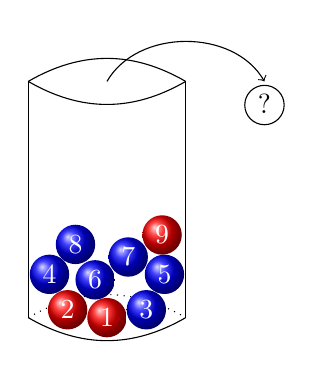
\begin{tikzpicture}
		\draw (0,0) -- (0,-3);
		\draw (2,0) -- (2,-3);
		\draw (0,-3) to [bend right] (2,-3);
		\draw[dotted] (0,-3) to [bend left] (2,-3);
		\draw (0,0) to [bend right] (2,0);
		\draw (0,0) to [bend left] (2,0);
		
		\begin{scriptsize}
		\shade [ball color=red] (1,-3) circle (0.25cm);
		\shade [ball color=red] (0.5,-2.9) circle (0.25cm);
		\shade [ball color=blue] (1.5,-2.9) circle (0.25cm);
		\shade [ball color=blue] (0.27,-2.45) circle (0.25cm);
		\shade [ball color=blue] (1.73,-2.45) circle (0.25cm);
		\shade [ball color=blue] (0.85,-2.52) circle (0.25cm);
		\shade [ball color=blue] (1.27,-2.23) circle (0.25cm);
		\shade [ball color=blue] (0.6,-2.07) circle (0.25cm);
		\shade [ball color=red] (1.7,-1.95) circle (0.25cm);
		\end{scriptsize}
		\node[white] at (1,-3) (1) {1};
		\node[white] at (0.5,-2.9) (2) {2};
		\node[white] at (1.5,-2.9) (3) {3};
		\node[white] at (0.27,-2.45) (4) {4};
		\node[white] at (1.73,-2.45) (5) {5};
		\node[white] at (0.85,-2.52) (6) {6};
		\node[white] at (1.27,-2.23) (7) {7};
		\node[white] at (0.6,-2.07) (8) {8};
		\node[white] at (1.7,-1.95) (9) {9};
		
		\draw[->] (1,0) to [bend left=60] (3,0);
		\draw (3,-0.3) circle (0.25cm);
		\node at (3,-0.29) (a) {?};
	\end{tikzpicture}
\end{document}
%	\caption{Verteilung zu \propref{2_2_6}} 
    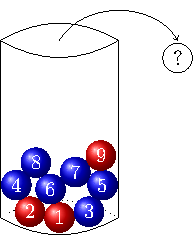
\includegraphics{../../Material/urne_mit_kugeln.pdf}
    \captionof{figure}{Urnenmodell} % needs \usepackage[font=small,labelfont=bf]{caption}
\end{center}

\subsection{Urnenmodell mit Zurücklegen: Multinomial-Verteilung}

Gegeben: Urne mit $N$ Kugeln, verschiedenfarbig mit Farben aus $E$, $\abs{E} \ge 2$ 

Ziehe: $n$ Stichproben/Kugeln, wobei nach jedem Zug die Kugel wieder zurückgelegt wird. Uns interessiert die Farbe in jedem Zug, setze also
\begin{align}
	\Omega = E^n \und \sigF = \pows(\Omega) \notag
\end{align}
Zur Bestimmung einer geeigneten Wahrscheinlichkeitsmaßes, nummerieren wir die Kugeln mit $1,\dots, N$, so dass alle Kugeln der Farbe $a \in E$ eine Nummer aus $F_{a} \subset \set{1,\dots, N}$ tragen. Würden wir die Nummern notieren, so wäre
\begin{align}
	\overline{\Omega} = \set{1,\dots, N}^n \und \overline{\sigF} = \pows(\overline{\Omega})\notag
\end{align}
und wir könnten die Gleichverteilung $\overline{\probp} = \Gleich(\overline{\Omega})$ als Wahrscheinlichkeitsmaß für einem einzelnen Zug verwenden. Für den Übergang zu $\Omega$ konstruieren wir  Zufallsvariablen. Die Farbe im $i$-ten Zug wird beschrieben durch
\begin{align*}
	X_i: \overline{\Omega} \to E \mit \overline{\omega} = \left( \overline{\omega}_1, \dots, \overline{\omega}_n \right) \mapsto a \text{ falls } \overline{\omega}_i \in F_a\\
	\intertext{Der Zufallsvektor}
	X = (X_1, \dots, X_n): \overline{\Omega} \to \Omega\\
   \intertext{beschreibt dann die Abfolge der Farben. Für jedes $\omega \in \Omega$ gilt dann}
	\set{X = \omega} = F_{\omega_1} \times \cdots \times F_{\omega_n} = \bigtimes_{i=1}^{n} F_{\omega_i}\\
	\intertext{und damit}
	\probp(\set{\omega}) 
	&= \overline{\probp}(X^{-1}(\set{\omega})) = \probp(X=\omega)\\
	&= \frac{\abs{F_{\omega_1}} \cdots \abs{F_{\omega_n}}}{\abs{\overline{\Omega}}}\\
	&= \prod_{i=1}^{n} \frac{\abs{F_{\omega_i}}}{N} =: \prod_{i=1}^{n} \rho(\omega_i)
\end{align*}
Zähldichten, die sich als Produkt von Zähldichten schreiben lassen, werden auch als \begriff{Produktdichten} bezeichnet ($\nearrow$  \cref{sec_unabhangigkeit}). %TODO ref?!?!?!

Sehr oft interessiert bei einem Urnenexperiment nicht die Reihenfolge der gezogenen Farben, sondern nur die Anzahl der Kugeln in Farbe $a \in E$ nach $n$ Zügen. Dies enspricht
\begin{align*}
	\hat{\Omega} 
	= \set{k = (k_a)_{a \in E} \in \N_{0}^{\abs{E}} \colon \sum_{a \in E} k_a = n}
	\und \hat{\sigF} = \pows\brackets{\hat{\Omega}}\\
	\intertext{Den Übergang $\Omega \to \hat{\Omega}$ beschreiben wir durch die Zufallsvariablen}
	Y_a(\omega): \Omega \to \N_{0} \mit \omega &= (\omega_1,\dots, \omega_n)\mapsto \sum_{a \in E} \indi_{\set{a}}(\omega_i)\\
	\intertext{und}
	Y = \brackets{Y_a}_{a\in E}: \Omega \to \hat{\Omega} &= \set{k = (k_a)_{a\in E}\colon \sum_{a \in E} k_a = n}
\end{align*}

% % % % % % % % % % % % % % % % % % % % 4th lecture % % % % % % % % % % % % % % % % % % % % % % %

Wir erhalten
\begin{align*}
	\probp(Y = k) &= \probp(Y_a = k_a, \enskip a \in E)\notag\\
	&= \sum_{\omega \in \Omega: Y(\omega) = k} \prod_{i=1}^{n} \rho(\omega_i)\notag\\
	&= \sum_{\omega \in \Omega: Y(\omega) = k} \prod_{a \in E} \rho(a) 
	&= \binom{n}{(k)_{a\in E}} 
%	\begin{pmatrix}
%	n \\
%	(k)_{a\in E}
%	\end{pmatrix}
	\prod_{a \in E} \rho(a)^{k_a},\\
	\intertext{wobei}
	\binom{n}{(k_1, \dots, k_l)} 
	&= 
	\begin{cases}
	\frac{n!}{k_1 ! \, k_2 ! \cdots k_l !} \sum_{i=1}^{l} k_i = n\\
	0 & \sonst
	\end{cases}
\end{align*}
der \begriff{Multinomialkoeffizient} ist, welcher die Anzahl der Möglichkeiten beschreibt, $n$ Objekte in $l$ Gruppen aufzuteilen, so dass Gruppe $i$ gerade $k_i$ Objekte beinhaltet.

\begin{definition}
	Sei $l > 2, p = (p_1, \dots, p_l)$ eine Zähldichte und $n \in \N$, dann heißt die Verteilung auf \\
	$\set{k = (k_i)_{i=1,\dots,l} \in \N_{0}^{l} : \sum_{i=1}^{l} k_i = n}$ mit Zähldichte
	\begin{align}
		m((k_1,\dots,k_l)) = \binom{n}{k_1, \dots, k_l}\prod_{i=1}^{l} p_i^{k_i}\notag
	\end{align}
	\begriff{Multinomialverteilung mit Parametern $n$ und $p$}. Wir schreiben auch $\Multi(n,p)$.
\end{definition}

\begin{example}
	Eine Urne enthalte nur schwarze ``$1$'' und weiße ``$0$'' Kugeln, d.h. $E=\set{0,1}$, und es sei $\rho(1) = p$ gerade die Proportion der schwarzen Kugeln (= Wahrscheinlichkeit bei einem Zug schwarz zu ziehen), dann ist Wahrscheinlichkeit in $n$ Zügen $k$-mal schwarz zu ziehen:
	\begin{align}
		\binom{n}{k}\prod_{i=0,1} \rho(i)^{k_i} = \binom{n}{k} p^k (1-p)^{n-k}.\notag
	\end{align}
	Ein solches (wiederholtes) Experiment mit nur zwei möglichen Ereignissen und fester Wahrscheinlichkeit $p \in [0,1]$ für eines der Ergebnisse nennen wir auch \begriff{(wiederholtes) Bernoulliexperiment}.
\end{example}

\begin{definition}
	Sei $p \in [0,1]$ und $n \in \N$, dann heißt die Verteilung mit Zähldichte
	\begin{align}
		\rho(k) = \binom{n}{k}p^k (1-p)^{n-k} \mit k \in \set{0,1,\dots,n}.\notag
	\end{align}
	\begriff{Binomialverteilung auf $\set{0, \dots,n}$ mit Parameter $p$} (auch \begriff{Erfolgswahrscheinlichkeit}). Wir schreiben auch $\Bin(n,p)$. Im Fall $n = 1$ nennen wir die Verteilung mit Zähldichte
	\begin{align}
		\rho(0) = 1-p \und \rho(1) = p\notag
	\end{align}
	auch \begriff{Bernoulliverteilung mit Parameter $p$} und schreiben $\Ber(p)$.
\end{definition}
\underline{Urnenmodell ohne Zurücklegen}: \begriff{Hypergeometrische Verteilung}\\
Gegeben: Urne mit $N$ Kugeln verschiedener Farben aus $E$,
\begin{align}
	\abs{E} \ge 2.\notag
\end{align}
Es werden $n \le N$ Stichproben entnommen, wobei die gezogenen Kugeln werde \emph{nicht} in die Urne zurückgelegt.

\subsection{Urnenmodell ohne Zurücklegen: Hypergeometrische Verteilung}
Gegeben: Urne mit $N$ Kugeln verschiedener Farben aus $E$, $\abs{E} \ge 2$. Es werden $n \le N$ Stichproben entnommen, wobei die gezogenen Kugeln werde \emph{nicht} in die Urne zurückgelegt.
\begin{example}
	Eine Urne enthalte $S$ schwarze ``$1$'' und $W$ weiße Kugeln ``$0$'' Kugeln, $(E = \set{0,1}, S + W =N)$. Dann ist die Wahrscheinlichkeit in $n$ Zügen ohne Zurücklegen gerade $s$ schwarze und $w$ weiße Kugeln zu ziehen
	\begin{align}
		\rho(w) = \frac{\binom{W}{w}\binom{S}{s}}{\binom{N}{n}}, \quad 0 \le s \le S, 0 \le w \le W, s+w = n, S+W = N.\notag
	\end{align}
\end{example}

\begin{proof}
	Hausaufgabe! %TODO add number later
\end{proof}

\begin{definition}
	Seinen $N \in \N, W \le N, n \le N$, dann heißt die Verteilung auf $\set{0,\dots,n}$ mit Zähldichte
	\begin{align}
		\rho(w) = \frac{\binom{wW}{w}\binom{N-W}{n-w}}{\binom{N}{n}}, \quad w = \max\set{0,n=N+W}, \dots, \min\set{W,n},\notag
	\end{align}
	die \begriff{Hypergeometrische Verteilung} mit Parametern $N,W,n$. Wir schreiben $\Hyper(N,W,n)$.
\end{definition}

\section{Poisson-Approximation und \person{Poisson}-Verteilung}

$\Bin(n,p)$ ist zwar explizit und elementar definiert, jedoch für große $n$ mühsam auszuwerten. Für seltene Ereignisse ($n$ groß, $p$ klein) verwende daher:
\begin{proposition}[Poisson-Approximation]
	Sei $\lambda > 0$ und $(p_n)_{n\in\N}$ eine Folge in $[0,1]$ mit
	\begin{align}
		np_n \to \lambda,\quad n \to \infty.\notag
	\end{align}
	Dann gilt $\forall k \in \N_0$ für die Zähldichte der $\Bin(n,p_n)$-Verteilung
	\begin{align}
		\lim_{n \to \infty} \binom{n}{k}p_n^k(1-p)^{n-k} = e^{-\lambda} \frac{\lambda^k}{k!}.\notag
	\end{align}
\end{proposition}
\begin{proof}
	Sei $k \in \N_{0}$ fix, dann
	\begin{align} %TODO fix this alignment mess and the tags!
		\binom{n}{k} = \frac{n!}{k!(n-k)!} &= \frac{n^k}{k!}\frac{n(n-1)\cdots(n-k+1)}{n^k}\notag\\
		&= \frac{n^k}{k!}\cdot 1 \cdot (1-\frac{1}{n}\cdots \frac{k-1}{n})\notag\\
		\overset{n \to \infty}&{\sim} \frac{n^k}{k!},\notag
	\end{align}
	wobei $a(l) \overset{n \to \infty}{\sim} b(l) \Leftrightarrow \frac{a(l)}{b(l)} \xrightarrow{n\to \infty} 1$. Damit
	\begin{align}
		\binom{n}{k}p^k (1-p)^{n-k} \overset{n \to \infty}&{\sim} \frac{n^k}{k!}p_n^k(1-p_n)^{n-k}\notag\\
		\overset{n \to \infty}&{\sim} \frac{\lambda^k}{k!}(1-p_n)^n\notag\\
		&= \frac{\lambda^n}{k!}\brackets{1 - \frac{np_n}{n}}^n\notag\\
		&\xrightarrow{n \to \infty} \frac{\lambda^n}{k!}e^{-\lambda}.\notag
	\end{align}
\end{proof}
Der erhaltene Grenzwert liefert die Zähldichte auf $\N_{0}$, denn 
\begin{align}
	\sum_{k=0}^{\infty}\frac{\lambda^k}{k!}e^{-\lambda} = e^{-\lambda}\sum_{k=0}^{\infty}\frac{\lambda^{k}}{k!} = e^{-\lambda}e^{\lambda} = 1\notag
\end{align}

\begin{definition}
	Sei $\lambda >0$. Dann heißt das auf $(\N_{0}, \probp(\N_{0}))$ definierte Wahrscheinlichkeitsmaß mit
	\begin{align}
		\probp(\set{k}) = \frac{\lambda^k}{k!}e^{-\lambda} \quad k \in \N_{0},\notag
	\end{align}
	\begriff{Poissonverteilung mit Parameter $\lambda$}. Schreibe $\Pois(\lambda)$.
\end{definition}
Die Poissonverteilung ist ein natürliches Modell für die Anzahl von zufälligen, seltenen Ereignissen (z.B. Tore im Fußballspiel, Schadensfälle einer Versicherung, ...).
\chapter[Bedingte Wkeiten und (Un-)abbhängigkeit]{Bedingte Wahrscheinlichkeiten und (Un)-abbhängigkeit}
\chaptermark{Bedingte Wahrscheinlichkeiten und (Un)-abbhängigkeit}
\section{Bedingte Wahrscheinlichkeiten}
\begin{example}
	\proplbl{3_1_1}
	Das Würfeln mit zwei fairen, sechsseitigen Würfeln können wir mit 
	\begin{align}
		\O = \set{(i,j) \colon i,j \in \set{1,\dots,6}}\notag
	\end{align}
	und $\P = \Gleich(\O)$. Da $\abs{\O} = 36$ gilt also
	\begin{align}
		\P(\set{\omega}) = \frac{1}{36} \quad \forall \omega \in \O.\notag
	\end{align}
	Betrachte das Ereignis
	\begin{align}
		A = \set{(i,j) \in \O \colon i + j = 8},\notag
	\end{align}
	dann folgt
	\begin{align}
		\P(A) = \frac{5}{36}.\notag
	\end{align}
	Werden die beiden Würfe nacheinander ausgeführt, so kann nach dem ersten Wurf eine Neubewertung der Wahrscheinlichkeit von $A$ erfolgen.\\
	Ist z.B.
	\begin{align}
		B = \set{(i,j) \in \O, i = 4}\notag
	\end{align}
	eingetreten, so kann die Summe $8$ nur durch eine weitere $4$ realisiert werden, also mit Wahrscheinlichkeit
	\begin{align}
		\frac{1}{6} = \frac{\abs{A \cap B}}{\abs{B}}.\notag 
	\end{align}
	Das Eintreten von $B$ führt also dazu, dass das Wahrscheinlichkeitsmaß $\P$ durch ein neues Wahrscheinlichkeitsmaß $\P_{B}$ ersetzt werden muss. Hierbei sollte gelten:
	\begin{align}
		 &\text{Renormierung: }\P_{B} = 1\label{Renorm}\tag{R}\\
		 &\text{Proportionalität: Für alle} A \subseteq \F \mit A \subseteq B \text{ gilt }
		 \P_{B}(A) = c_B \P(A) \text{ mit einer Konstante } c_B.\label{Prop}\tag{P}
    \end{align}
\end{example}

\begin{lemma}
	Sei $(\O, \F, \P)$ Wahrscheinlichkeitsraum und $B \in \F$ mit $\P(B) > 0$. Dann gibt es genau ein Wahrscheinlichkeitsmaß $\P_B$ auf $(\O, \F)$ mit den Eigenschaften \eqref{Renorm} und \eqref{Prop}. Dieses ist gegeben durch
	\begin{align}
		\P_{B}(A) = \frac{\P(A\cap B)}{\P(B)} \quad \forall A \in \F.\notag
	\end{align}
\end{lemma}

\begin{proof}
	Offenbar erfüllt $\P_{B}$ wie definiert \eqref{Renorm} und \eqref{Prop}. Umgekehrt erfüllt $\P_{B}$ \eqref{Renorm} und \eqref{Prop}. Dann folgt für $A \in \F$:
	\begin{align}
		\P_{B}(A) = \P_{B}(A\cap B) + \underbrace{\P_{B}(A\setminus B)}_{= 0, \text{ wegen } \eqref{Renorm}} \overset{\eqref{Prop}}{=} c_B \P(A \cap B).\notag
	\end{align}
	Für $A=B$ folgt zudem aus \eqref{Renorm}
	\begin{align}
		1 = \P_{B}(B) = c_B \P(B)\notag
	\end{align}
	also $c_B = \P(B)^{-1}$.
\end{proof}

% % % % % % % % % % % % % % % % % % % % % % % % % % % 5th lecture % % % % % % % % % % % % % % % % % % % % % % % % % % %

\begin{definition}
	\proplbl{3_1_3}
	Sei $(\O, \F, \P)$ Wahrscheinlichkeitsraum und $B \in \F$ mit $\P(B) > 0$. Dann heißt
	\begin{align*}
		\P(A\mid B) := \frac{\P(A\cap B)}{\P(B)} \mit A\in \F
	\end{align*}
	die \begriff{bedingte Wahrscheinlichkeit von $A$ gegeben $B$}.
	Falls $\P(B) = 0$, setze
	\begin{align*}
		\P(A \mid B) = 0 \qquad \forall A \in \F
	\end{align*}
\end{definition}

\begin{example} %TODO ref
	In der Situation \propref{3_1_1} gilt % 
	\begin{align*}
		A \cap B = \set{(4,4)}
		\intertext{und damit}
		\P(A \mid B) = \frac{\P(A\cap B)}{\P(B)} = \frac{\frac{1}{36}}{\frac{1}{6}} = \frac{1}{6}
	\end{align*}
\end{example}

Aus \propref{3_1_3} ergibt sich
\begin{lemma}[Multiplikationsformel]
	\proplbl{3_1_4}
	Sei $(\O, \F, \P)$ ein Wahrscheinlichkeitsraum und $A_1, \dots, A_n \in \F$. Dann gilt
	\begin{align*}
		\P(A_1 \cap \cdots \cap A_n) = \P(A_1) \P(A_2 \mid A_1) \dots \P(A_n \mid A_1 \cap \cdots \cap A_{n-1})
	\end{align*}
\end{lemma}

\begin{proof}
	Ist $\P(A_1 \cap \dots \cap A_n) = 0$, so gilt auch $\P(A_n \mid \bigcap_{i=1}^{n-1} A_i) = 0$. Andernfalls sind alle Faktoren der rechten Seite ungleich Null und
	\begin{align*}
		\P(A_1) \P(A_2 \mid A_1) \dots \P(A_n \mid \bigcap_{i=1}^{n-1} A_i) \\
		&= \P(A_1) \cdot \frac{\P(A_1 \cap A_2)}{\P(A_1)} \dots \frac{\P(\bigcap_{i=1}^{n} A_i)}{\P(\bigcap_{i=1}^{n-1}A_i)} \\
		&= \P(\bigcap_{i=1}^n A_i)	
	\end{align*}
\end{proof} %TODO add ref.

Stehen die $A_i$ in \propref{3_1_4} in einer (zeitlichen) Abfolge, so liefert Formel einen Hinweis wie Wahrscheinlichkeitsmaße für \begriff{Stufenexperimente} konstruiert werden können. Ein \emph{Stufenexperiment} aus $n$ nacheinander ausgeführten Teilexperimenten lässt sich als \begriff{Baumdiagramm} darstellen.

%(done) Baumdiagramm
\begin{center}
		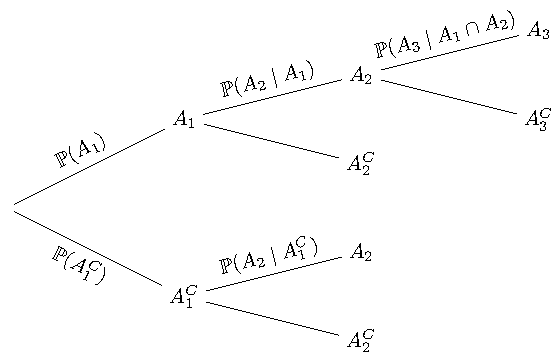
\includegraphics{./tikz/baum_1.pdf}
		\captionof{figure}{\cref{3_1_4}} %\propref{3_1_4}} funktioniert nicht
\end{center}

\begin{proposition}[Konstruktion des Wahrscheinlichkeitsmaßes eines Stufenexperiments]
	\proplbl{3_1_6}
	Gegeben seinen $n$ Ergebnisräume $\O_i = \set{\omega_i (1), \dots, \omega_i (k)}, k \in \N \cup \set{\infty}$ und es sei $\O = \bigtimes_{i = 1}^n \O_i$ der zugehörige Produktraum. Weiter seinen $\F_i$ $\sigma$-Algebren auf $\O_i$ und $\F = \bigotimes_{i=1}^n \F_i$ die Produkt-$\sigma$-Algebra auf $\O$. Setze $\omega = (\omega_1,\dots,\omega_n)$ und
	\begin{align*}
		[\omega_1,\dots,\omega_m]:= \set{\omega_1}\times \dots \times \set{\omega_m} \times \O_{m+1} \times \cdots \times \O_{n},\quad m\le n\\
		\P(\set{\omega_m}[\omega_1,\dots,\omega_{m-1}])
	\end{align*}
	für die Wahrscheinlichkeit in der $m$-ten Stufe des Experiments $\omega_m$ zu beobachten, falls in den vorausgehenden Stufen $\omega_1,\dots,\omega_{m-1}$ beobachten wurden. Dann definiert
	\begin{align*}
		\P(\set{\omega}) := \P(\set{\omega_1}) \prod_{m=2}^{n}\P\brackets{\set{\omega_m} \mid [\omega_1, \dots, \omega_{m-1}]}
		%(done) maybe wrong here. check
	\end{align*}
	ein Wahrscheinlichkeitsmaß auf $(\O, \F, \P)$.
\end{proposition}
\begin{proof}
	Nachrechnen!
\end{proof}

\begin{example}[\person{Polya}-Urne]
	Gegeben sei eine Urne mit $s$ schwarzen und $w$ weißen Kugeln. Bei jedem Zug wird die  gezogene Kugel zusammen mit $c\in \N_0 \cup \set{-1}$ weiteren Kugeln derselben Farbe zurückgelegt.
	\begin{itemize} %TODO seen both in chapter 2.2, but big bracket behind.
		\item $c=0$: Urnenmodell mit Zurücklegen
		\item $c=-1$: Urnenmodell ohne Zurücklegen
	\end{itemize}
	Beide haben wir schon in Kapitel 2.2 gesehen.\\
	Sei deshalb $c\in \N$. (Modell für zwei konkurrierende Populationen) Ziehen wir $n$-mal, so haben wir ein $n$-Stufenexperiment mit 
	\begin{align*}
		\O = \set{0,1}^n \mit \text{ 0 = ``weiß'', 1 = ``schwarz''} \quad (\O_i = \set{0,1})
		\intertext{Zudem gelten im ersten Schritt}
		\P(\set{0}) = \frac{w}{s+w} \und \P(\set{1}) = \frac{s}{s+w}
		\intertext{sowie}
		\P(\set{\omega_m} \mid [\omega_1, \dots \omega_{m-1}]) = 
		\begin{cases} %(done) fix brackets!
		\frac{w+c \brackets{m-1 - \sum_{i=1}^{m-1}\omega_i}}{s+w+c(m-1)} & \omega_m = 0\\
		\frac{s + c\sum_{i=1}^{m-1}\omega_i}{s+w+c(m-1)} & \omega_m = 1
		\end{cases}
	\end{align*}
	Mit \propref{3_1_6} folgt als Wahrscheinlichkeitsmaß auf $(\O, \pows(\O))$
	\begin{align*}
		\P(\set{(\omega_1, \dots, \omega_n)}) &= \P(\set{\omega_1}) \prod_{m=2}^n \P(\set{\omega_m}\mid [\omega_1,\dots,\omega_{m-1}]) \\
		&=\frac{\prod_{i=0}^{l-1}(s+c \cdot i)\prod_{i=0}^{n-l-1}(w + c \cdot j)}{\prod_{i=0}^n (s+w+c \cdot i)} \mit l=\sum_{i=1}^n \omega_i.
		\intertext{Definiere wir nun die Zufallsvariable}
		S_n:\O &\to \N_0 \mit (\omega_1, \dots, \omega_n) \mapsto \sum_{i=1}^n \omega_i
		\intertext{welche die Anzahl der gezogenen schwarzen Kugeln modelliert, so folgt}
		\P(S_n = l) &= \binom{n}{l} \frac{\prod_{i=0}^{l-1}(s+c \cdot i) \prod_{j=0}^{n-l-1}(w + c \cdot j)}{\prod_{i=0}^n(s+w+c \cdot i)}
		\intertext{Mittels $a:= \sfrac{s}{c},b:= \sfrac{w}{c}$ folgt}
		\P(S_n = l) &= \binom{n}{l} \frac{\prod_{i=0}^{l-1}(-a-i)\prod_{j=0}^{n-l-1}(-b-j)}{\prod_{i=0}^n (-a-b-i)} = \frac{\binom{-a}{l}\binom{-b}{n \cdot l}}{\binom{-a-b}{n}}\\ &\mit l \in \set{0,\dots,n} 
	\end{align*}
	Dies ist die \begriff{\person{Polya}-Verteilung} auf $\set{0,\dots,n}, n \in \N$ mit Parametern $a,b > 0$.
\end{example}

\begin{example}
	Ein Student beantwortet eine Multiple-Choice-Frage mit 4 Antwortmöglichkeiten, eine davon ist richtig. Er kennt die richtige Antwort mit Wahrscheinlichkeit $\sfrac{2}{3}$. Wenn er diese kennt, so wählt er diese aus. Andernfalls wählt er zufällig (gleichverteilt) eine Antwort. Betrachte
	\begin{align*}
		W &= \set{\text{richtige Antwort gewusst}}\\
		R &= \set{\text{Richtige Antwort gewählt}}
		\intertext{Dann gilt}
		\P(W) &= \frac{2}{3}, \P(R \mid W) = 1, \P(R \mid W^C) = \frac{1}{4} 
	\end{align*}
	Angenommen, der Student gibt die richtige Antwort. Mit welcher Wahrscheinlichkeit hat er diese gewusst? $\longrightarrow \P(W\mid R) = \text{ ?}$
\end{example}

\begin{proposition}
	\proplbl{3_1_9}
	Sei $(\O, \F, \P)$ Wahrscheinlichkeitsraum und $\O = \bigcup_{i \in I} B_i$ eine höchstens abzählbare Zerlegung in paarweise disjunkte Ereignisse $B_i \in \F$.
	\begin{enumerate} %TODO set itemize references. or use enumerate?
		\item \emph{Satz von der totalen Wahrscheinlichkeit:} Für alle $A \in \F$ gilt
		\begin{align*}
			\P(A) = \sum_{i\in I} \P(A\mid B_i)\P(B_i) \label{eq:totWkeit}\tag{totale Wahrscheinlichkeit}
		\end{align*} 
		\item \emph{Satz von \person{Bayes}:} Für alle $A \in \F$ mit $\P(A) > 0$ und alle $k \in I$
		\begin{align*}
			\P(B_k \mid A) = \frac{\P(A \mid B_k) \P(B_k)}{\sum_{i\in I}\P(A\mid B_i)\P(B_i)} \label{eq:bayes}\tag{Bayes}
		\end{align*}
	\end{enumerate}
\end{proposition}

\begin{proof}
	\begin{enumerate}
		\item Es gilt:
		\begin{align*}
			\sum_{i\in I} \P(A\mid B_i)\P(B_i) \defeq \sum_{i\in I}\frac{\P(A \cap B_i)}{\P(B_i)}\P(B_i) = \sum_{i\in I} \P(A \cap B_i) \overset{\sigma-Add.}{=} \P(A)
		\end{align*}
		\item 
		\begin{align*}
			\P(B_k \mid A) \defeq \frac{\P(A \cap B_k)}{\P(A)} \defeq \frac{\P(A \mid B_k)\P(B_k)}{\P(A)}
		\end{align*}
		also folgt (b) aus (a). %TODO add refs
	\end{enumerate}
\end{proof}

\begin{example}
	In der Situation von \propref{3_1_3} folgt mit \propref{3_1_9} \eqref{eq:totWkeit}
	\begin{align*}
		\P(R) &= \P(R \mid W)\P(W) + \P(R\mid W^C)\P(W^C)\\
		&= 1 \cdot \frac{2}{3} + \frac{1}{4} \frac{1}{3} = \frac{3}{4}
		\intertext{und mit \propref{3_1_9} \eqref{eq:bayes}} %Bayes
		\P(W \mid R) &= \frac{\P(R \mid W)\P(W)}{\P(R)} = \frac{1 \cdot \frac{2}{3}}{\frac{3}{4}} = \frac{8}{9} \text{ für die gesuchte Wahrscheinlichkeit.}
	\end{align*} %(done) compile as pdf and include it. not working.
	\begin{center}
			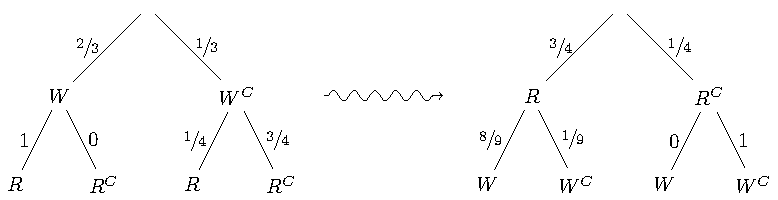
\includegraphics{./tikz/baum_2.pdf}
			\captionof{figure}{\cref{3_1_3}} %\propref{3_1_3} funktioniert nicht
	\end{center}
\end{example}
\section{(Un)abhängigkeit} \label{sec:unabhangigkeit}
In vielen Fällen besagt die Intuition über verschiedene Zufallsexperimente / Ereignisse, dass diese sich \emph{nicht} gegenseitig beeinflussen. Für solche $A,B \in \F$ mit $\P(A) > 0, \P(B) > 0$ sollte gelten
\begin{align*}
\P(A\mid B) = \P(A), \quad \P(B\mid A) = \P(B).
\end{align*}

\begin{definition}[(Stochastische) Unabhängigkeit]
	\proplbl{3_2_11}
	Sei $(\O, \F, \P)$ Wahrscheinlichkeitsraum. Zwei Ereignisse $A,B \in \F$ heißt \begriff{(stochastisch) unabhängig bezüglich $\P$}, falls
	\begin{align*}
		\P(A\cap B) = \P(A)\P(B).
	\end{align*}
	Wir schreiben auch $A \upmodels B$.
\end{definition}
\begin{example}
	Würfeln mit 2 fairen, sechsseitigen Würfeln:
	\begin{align*}
	\O &= \set{(i,j) \mid i,j \in\set{1,\dots,n}},\quad \F = \pows(\O), \quad \P = \Gleich(\O)
	\intertext{Betrachte}
	A:= \set{(i,j) \in \O, i \text{ gerade}}\\
	B:= \set{(i,j) \in \O, j \le 2}.
	\end{align*}
	In diesem Fall, erwarten wir intuitiv Unabhängigkeit von $A$ und $B$.\\
	In der Tat ist % start using \P instead of \P!
	\begin{align*}
	\P(A) = \frac{1}{2}, \quad \P(B) = \frac{1}{3} \und \P(A\cap B) = \frac{1}{6}
	\intertext{was}
	\P(A \cap B) = \P(A) \P(B)
	\intertext{erfüllt}
	\end{align*}
	Betrachte nun
	\begin{align*}
	C&:= \set{(i,j) \in \O \mid i + j = 7}\\
	D&:= \set{(i,j) \in \O \mid i = 6}
	\intertext{dann gilt}
	\P(C) = \frac{1}{6}, \quad \P(D) = \frac{1}{6}
	\intertext{und wegen $C \cap D = \set{(6,1)}$ folgt}
	\P(C\cap D) = \frac{1}{36} = \frac{1}{6} \frac{1}{6} = \P(C) \cdot \P(D)
	\end{align*}
	$C$ und $D$ sind also \emph{stochastisch} unabhängig, obwohl eine kausale Abhängigkeit vorliegt!
\end{example}

\begin{definition}[Unabhängigkeit bezüglich $\P$]
	Sei $(\O, \F, \P)$ Wahrscheinlichkeitsraum und $I \neq \emptyset$ endliche Indexmenge. Dann heißt die Familie $(A_i)_{i \in I}$ von Ereignissen in $\F$ \begriff{unabhängig bezüglich $\P$}, falls für alle $J \subseteq I, J \neq \emptyset$ gilt:
	\begin{align*}
		\P\brackets{\bigcap_{i\in J}A_i} = \prod_{i\in J} \P(A_i)
	\end{align*}
	Offensichtlich impliziert die Unabhängigkeit einer Familie die paarweise Unabhängigkeit je zweier Familienmitglieder nach \propref{3_2_11}. Umgekehrt gilt dies nicht!
\end{definition}

\begin{example}[Abhängigkeit trotz paarweiser Unabhängigkeit]
	Betrachte zweifaches Bernoulliexperiment mit Erfolgswahrscheinlichkeit $\sfrac{1}{2}$, d.h.
	\begin{align*}
		\O = \set{0,1}^2, \quad \F = \pows(\O), \quad \P = \Gleich(\O)
		\intertext{sowie}
		A &= \set{1}\times \set{0,1} \qquad \text{(Münzwurf: erster Wurf ist Zahl)}\\
		B &= \set{0,1}\times \set{1} \qquad \text{(Münzwurf: zweiter Wurf ist Zahl)}\\
		C &= \set{(0,0), (1,1)} \qquad \text{(beide Würfe haben selbes Ergebnis)}
	\end{align*}
	Dann gelten
	\begin{align*}
		\P(A) = \frac{1}{2} = \P(B) = \P(C)
		\intertext{und}
		\P(A\cap B) = \P(\set{(1,1)}) = \frac{1}{4} = \P(A)\P(B)\\
		\P(A\cap C) = \P(\set{(1,1)}) = \frac{1}{4} = \P(A)\P(C)\\
		\P(B\cap C) = \P(\set{(1,1)}) = \frac{1}{4} = \P(B)\P(C)
	\end{align*}
	also paarweise Unabhängigkeit.\\
	Aber
	\begin{align*}
	\P(A\cap B \cap C) = \P(\set{(1,1)}) = \frac{1}{4} \neq \P(A)\P(B)\P(C)
	\end{align*}
	und $A,B,C$ sind \emph{nicht} stochastisch unabhängig.
\end{example}

\begin{definition}[Unabhängige $\sigma$-Algebren]
	\proplbl{3_2_15}
	% started using \O for \Omega and \E for this special generating set E_i
	Seien $(\O, \F,\P)$ Wahrscheinlichkeitsraum, $I \neq \emptyset$ Indexmenge und $(E_i, \Gen_i)$ Messräume
	\begin{enumerate}
		\item Die Familie $\F_i \subset \F, i \in I$, heißen \begriff{unabhängig}, wenn für die $J \subseteq I, J \neq \emptyset, \abs{J} < \infty$ gilt
		\begin{align*}
			\P\brackets{\bigcap_{i \in J} A_i} = \prod_{i\in J} \P(A_i) \qquad \text{ für beliebige } A_i \in \F_i, i \in J
		\end{align*}
		\item Die Zufallsvariable $X_i: (\O, \F) \to (E_i, \Gen_i), i \in I$, heißen \begriff{unabhängig}, wenn die $\sigma$-Algebren
		\begin{align*}
		\sigma(X_i) = X^{-1}(\Gen_i) = \set{\set{X_i \in F} \colon F \in \Gen_i}, \quad i \in I
		\end{align*}
		unabhängig sind.
	\end{enumerate}
\end{definition}

\begin{lemma}[Zusammenhang der Definitionen]
	\proplbl{3_2_16}
	Sei $(\O,\F,\P)$ Wahrscheinlichkeitsraum, $I \neq \emptyset, A \in \F, i \in I$. 
	Die folgenden Aussagen sind äquivalent:
	\begin{enumerate}
		\item Die Ereignisse $A_i, i \in I$ sind unabhängig. 
		\item Die $\sigma$-Algebren $\sigma(A_i), i \in I$ sind unabhängig.
		\item Die Zufallsvariablen $\indi_{A_i}, i \in I$ sind unabhängig.
	\end{enumerate}
\end{lemma}
\begin{proof} %TODO add ref?
	Da die Unabhängigkeit über endliche Teilemengen definiert ist, können wir oBdA $I = \set{1, \dots, n}$ annehmen. 
	\begin{itemize}
		\item Da $\sigma(\indi_{A_i}) = \sigma(A_i)$ folgt die Äquivalenz von 2. und 3. direkt aus \propref{3_2_15}.
		\item Zudem ist 2. $\to$ 1. klar!
		\item Für 1 $\to$ 2. genügt es zu zeigen, dass
		\begin{align*}
			A_1, \dots, A_n \text{ unabhängig } &\Rightarrow B_1, \dots, B_n \text{ unabhängig mit } B_i \in \set{\emptyset, A_i, A_i^C, \O}.
			\intertext{Rekursiv folgt dies bereits aus}
			A_1,\dots, A_n \text{ unabhängig } &\Rightarrow B_1, A_2, \dots, A_n \text{ unabhängig mit } B_1 \in \set{\emptyset, A_1, A_1^C, \O}.
		\end{align*}
		Für $B_1 \in \set{\emptyset, A_1, \O}$ ist dies klar.\\
		Sei also $B_1 = A_1^C$ und $J \subseteq I, J \neq \emptyset$. Falls $1 \not \in J$, ist nichts zu zeigen. Sei $1 \in J$, dann gilt mit
		\begin{align*}
			A &= \bigcap_{i\in J, i \neq 1} A_i
			\intertext{sicherlich}
			\P\brackets{A_1^C \cap A} &= \P(A \setminus (A_1 \cap A))\\
			&= \P(A) - \P(A_1 \cap A)\\
			&= \prod_{i\in J\setminus \set{1}} \P(A_i) - \prod_{i\in J}(A_i)\\
			&= (1- \P(A_1))\prod_{i\in J\setminus \set{1}} \P(A_i)\\
			&= \P\brackets{A_1^C})\prod_{i\in J\setminus \set{1}} \P(A_i)
		\end{align*} 
	\end{itemize}
\end{proof}
Insbesondere zeigt \propref{3_2_16}, dass wir in einer Familie unabhängiger Ereignisse beliebig viele Ereignisse durch ihr Komplement, $\emptyset$ oder $\O$ ersetzen können, ohne die Unabhängigkeit zu verlieren.
\begin{proposition}
	\proplbl{3_2_17}
	Sei $(\O, \F, \P)$ Wahrscheinlichkeitsraum und $\F_i \subseteq \F, i \in I$, seien $\cap$-stabile Familien von Ereignissen. Dann gilt
	\begin{align*}
	\F_i, i \in I \text{ unabhängig } \iff \sigma(\F_i), i \in I \text{ unabhängig}. 
	\end{align*}
\end{proposition}
\begin{proof}
	oBdA sei $I = \set{1, \dots, n}$ und $\O \in \F_i, i \in I$.
	\begin{itemize}
		\item $\Leftarrow$: trivial, da $\F_i \subseteq \sigma(\F_i)$ und das Weglassen von Mengen erlaubt ist.
		\item $\Rightarrow$: zeigen wir rekursiv
		\begin{enumerate}
			\item Wähle $F_i \in \F_i, i = 2, \dots,n$ und defniere für $F \in \sigma(\F_i)$ die endlichen Maße
			\begin{align*}
				\mu(F) = \P\brackets{ F \cap F_2 \cap \cdots \cap F_n} \und \nu(F) = \P(F) \, \P(F_2) \, \dots \, \P(F_n)
			\end{align*}
			\item Da die Familien $\F_i$ unabhängig sind, gilt
			$\mu\mid_{\F_1} = \nu\mid_{\F_1}$.
			Nach dem Eindeutigkeitssatz für Maße (\propref{1_1_9}) folgt $\mu\mid_{\sigma(\F_1)} = \nu\mid_{\sigma(\F_1)}$ also
			\begin{align*}
				\P\brackets{ F \cap F_2 \cap \cdots \cap F_n} = \P(F) \P(F_2) \dots \P(F_n)
			\end{align*}
			für alle $F \in \sigma(\F_i)$ und $F_i \in \F_i, i = 1, \dots, n$. Da $\O \in \F_i$ für alle $i$ gilt die erhaltene Produktformel für alle Teilemengen $J \subseteq I$.\\
			Also sind
			\begin{align*}
			\sigma(\F_1), \F_2, \dots, \F_n \text{ unabhängig}
			\end{align*}
			\item Wiederholtes Anwenden von $1$ und $2$ liefert den Satz.
		\end{enumerate}
	\end{itemize}
\end{proof}
Mit \propref{3_2_17} folgen:
\begin{conclusion}
	\proplbl{3_2_18}
	Sei $(\O,\F,\P)$ Wahrscheinlichkeitsraum und
	\begin{align*}
		\F_{i,j} \subseteq \F, \quad 1 \le i \le n, 1 \le j \le m(i)
	\end{align*}
	unabhängige, $\cap$-stabile Familien.
	Dann sind auch
	\begin{align*}
		\G_i = \sigma(\F_{i,1}, \dots , \F_{i,m(i)}), \quad 1 \le i \le n
	\end{align*}
	unabhängig.
\end{conclusion}
\begin{conclusion}
	\proplbl{3_2_19}
	Sei $(\O,\F,\P)$ Wahrscheinlichkeitsraum und
	\begin{align*}
		X_{ij}: \O \to E, \quad 1 \le i \le n, 1 \le j \le m(i)
	\end{align*}
	unabhängige Zufallsvariablen. Zudem seien $f_i: E^{m(i)} \to \R$ messbar. Dann sind auch die Zufallsvariablen
	\begin{align*}
		f_i(X_{i,1}, \dots, X_{i,m(i)}), \quad 1 \le i \le n
	\end{align*}
	unabhängig.
\end{conclusion}
\begin{example}
	$X_1, \dots, X_n$ unabhängige reelle Zufallsvariablen. Dann sind auch
	\begin{align*}
	Y_1 = X_1, Y_2 = X_2 + \cdots + X_n
	\end{align*}
	unabhängig.
\end{example}
% % % % % % % % % % % % % % % % % 7th lecture % % % % % % % % % % % % % % % % % % %
\begin{proof}[\propref{3_2_18}]
	OBdA sei $\Omega \in \F_{i,j} \forall i,j$. Dann sind die Familien:
	\begin{align*}
		\F_i^{\cap} := \set{F_{i,1} \cap \dots \cap F_{i,m(i)} \mid F_{i,j} \in \F_{i,j}, 1 \le j \le m(i)}, 1 \le i \le n
	\end{align*}
	$\cap$-stabil, unabhängig und es gilt: $\F_{i,1}, \dots, \F_{i,m(i)} \subseteq \F_i^{\cap}$ ($\nearrow$ HA)! Nach \propref{3_2_17} sind auch $\sigma(\F_i^{\cap})$ unabhängig. Damit folgt die Behauptung, da $\sigma(\F_i^{\cap}) = \G_i$:
	\begin{align*}
		\F_{i,1}, \dots, \F_{i,m(i)} \subseteq \F_i^{\cap} \subseteq \sigma(\F_{i,1}, \dots, \F_{i,m(i)}) = \G_i\\
		\Rightarrow \G = \sigma(\F_{i,1}, \dots, \F_{i,m(i)}) \subseteq \sigma(\F_i^{\cap}) \subseteq \G_i.
	\end{align*}
\end{proof}
\begin{proof}[\propref{3_2_19}]
	Setze $\F_{i,j} = \sigma(X_{i,j})$ und $\G_i = \sigma(\F_{i,1}, \dots, \F_{i,m(i)})$, dann sind nach \propref{3_2_18} die $\G_i, i = 1,\dots,n$ unabhängig. Zudem ist
	\begin{align*}
	Y_i := f_i(X_{i,1}, \dots, X_{i,m(i)})
	\end{align*}
	$\G_i$ messbar, also $\sigma(Y_i) \subseteq \G_i$. Damit erben die $Y_i$ die Unabhängigkeit der $\G_i$.
\end{proof}
\begin{proposition}[Unabhängigkeit von Zufallsvariablen]
	\proplbl{3_2_21}
	$(\O, \F, \P)$ Wahrscheinlichkeitsraum und $X_1, \dots, X_n: (\O,\F) \to (E, \E)$ Zufallsvariablen. Dann sind die folgenden Aussagen äquivalent:
	\begin{enumerate}
		\item $X_1, \dots, X_n$ sind unabhängig \label{prop:unabhZV1}
		\item $\P(X_1 \in A_1, \dots, X_n \in A_n) = \prod_{i=1}^n \P(X_i \in A_i)\quad \forall A_1, \dots, A_n \in \E$. \label{prop:unabhZV2}
		\item Die gemeinsame Verteilung der $X_i$ entspricht dem Produktmaß der einzelnen Verteilungen \label{prop:unabhZV3}
		\begin{align*}
			\P_{X_1, \dots, X_n} = \bigotimes_{i=1}^n \P_{X_i}
		\end{align*}
	\end{enumerate}
\end{proposition}
\begin{proof}
	Per Ringschluss:
	\begin{enumerate} %TODO add labels
		\item[1 $\Rightarrow$ 2:] Seien $A_1, \dots, A_n\in E$ beliebig, dann gilt per Definition
		\begin{align*} % für Rechtecke
			\P_{X_1, \dots, X_n}(A_1 \times \dots \times A_n) &= \P(X_1 \in A_1, \dots, X_n \in A_n)\\
			&= \P\brackets{\bigcap_{i=1}^n \set{X_i \in A_i}}\\
			\overset{\text{unabh}}&{=} \prod_{i=1}^n \P(X_i \in A_i)\\
			&= \prod_{i=1}^n \P_{X_i}(A_i) = \brackets{\bigotimes_{i=1}^n \P_{X_i}} (A_1 \times \dots \times A_n) 
		\end{align*} 
		\item[2 $\Rightarrow$ 3:] Aus der obigen Rechnung sehen wir, dass 2 bereits 3 impliziert für alle Rechtecke: $\bigtimes_{i = 1}^n A_i$. Da die Familie der Rechtecke $\cap$-stabil ist und $\E^{\otimes n}$ erzeugt, folgt die Aussage aus dem Eindeutigkeitssatz für Maße \propref{1_1_9}.
		\item[3 $\Rightarrow$ 1:] Sei $J \subseteq \set{1,\dots,n}$ und setze
		\begin{align*}
			A_i &:= \begin{cases}
			\text{ beliebig }  &\text{ in }\E, i \in J\\
			E & i \notin J.
			\end{cases}
			\intertext{Dann}
			\P(X_i \in A_i, i \in J) &= \P(X_i \in A_i, i = 1, \dots,n)\\
			&= \prod_{i=1}^n \P(X_i \in A_i)\\
			&= \prod_{i\in J} \P(A_i \in A_i).
		\end{align*}
	\end{enumerate}
\end{proof}
\begin{example}
	Im Urnenmodell mit Zurücklegen hat der Vektor $X = (X_1, \dots, X_n)$ mit $X_i = $ Farbe im $i$-ten Zug als Zähldichte die Produktdichte der $X_i$. Die $X_1, \dots, X_n$ sind also unabhängig.
\end{example}
\subsection*{Konstruktion unabhängiger Zufallsvariablen}
Kapitel \ref{chapter1}: Zu beliebiger Wahrscheinlichkeitsverteilung $\P_X$ existiert Wahrscheinlichkeitsraum mit Zufallsvariable $X$ auf diesem Wahrscheinlichkeitsraum, so dass $X \sim \P_X$.
\begin{enumerate}
	\item Seien $\P_{X_1}, \dots, \P_{X_n}$ Wahrscheinlichkeitsverteilungen auf $(E, \E)$. Gibt es einen Wahrscheinlichkeitsraum $(\O, \F, \P)$ und Zufallsvariablen $X_1, X_2$ unabhängig, so dass $X_1 \sim \P_{X_1}$? \label{konstruktionunabh:ZV:qu_1}
	\item Wie kann ich beliebig (unendlich) viele unabhängige Zufallsvariablen konstruieren? \label{konstruktionunabh:ZV:qu_2}
\end{enumerate}
Wir beginnen mit \ref{konstruktionunabh:ZV:qu_1}:\\
Konstruiere zwei Wahrscheinlichkeitsräume $(\O_i, \F_i, \P_i), i = 1,2$ und Zufallsvariablen $X_1, X_2 \mit X_i \sim \P_{X_i}$. Auf dem Produktraum
\begin{align*}
	\O = \O_1 \times \O_2, \quad \F := \F_1 \otimes \F_2 \und \P = \P_1 \otimes \P_2
	\intertext{ definiere}
	X'_1: \O_1 \times \O_2 \to E\colon (\omega_1, \omega_2) \mapsto X_1(\omega_1)\\
	X'_2: \O_1 \times \O_2 \to E\colon (\omega_1, \omega_2) \mapsto X_2(\omega_2)
\end{align*}
Dann gilt für beliebige Ereignisse: $F_1, F_2 \in \E$
\begin{align*}
	\underbrace{\set{X'_1 \in F_1} \cap \set{X'_2 \in F_2}}_{\supseteq \O = \O_1 \times \O_2} = \underbrace{\set{X_1 \in F_1}}_{\supseteq \O_1} \times \underbrace{\set{X_2 \in F_2}}_{\supseteq \O_2} \in \F_1 \times \F_2
\end{align*}
und damit folgt die Messbarkeit der Abbildungen $X'_1, X'_2$, d.h. $X'_1, X'_2$ sind Zufallsvariablen auf $(\O, \F)$. Zudem gilt
\begin{align*}
	\P(X'_1 \in F_1, X'_2 \in F_2) &= \P_1 \otimes \P_2 \brackets{\set{X_1 \in F_1} \times \set{X_2 \in F_2}}\\
	&= \P_1 (X_1 \in F_1) \P_2(X_2 \in F_2),
	\intertext{also}
	\P(X'_i \in F_i) &= \P_i (X'_i \in F_i)
\end{align*}
sowie nach \propref{prop:Kolmo} $X'_1 \upmodels X'_2$.\\
Wenn $(\O_2, \F_1, \P_1) = (\O_2, \F_2, \P_2)$, so liefert die obige Konstruktion zwei unabhängige Zufallsvariablen auf einem Wahrscheinlichkeitsraum. Andernfalls können wir auf den Produktraum ausweichen und $X'_i$ anstelle von $X_i$ betrachten. Die obige Konstruktion lässt sich direkt auf \emph{endlich} viele Zufallsvariablen übertragen.\\
Zu \ref{konstruktionunabh:ZV:qu_2}: 
\begin{proposition}[Satz von \person{Kolmogorov}]
	\proplbl{prop:Kolmo}
	Sei $I$ beliebige Indexmenge und $(\O_i, \F_i, \P_i), i \in I$ Wahrscheinlichkeitsräume. Setze
	\begin{align*}
		\O_I &:= \bigtimes_{i \in I} \O_i = \set{\omega : I \to \bigcup_{i \in I} \O_i, \omega_i \in \O_i, i \in I}\\
		\F_I &:= \sigma( \pi^{-1} ( \F_i), i \in I)
	\end{align*}
	wobei $\pi_i : \O_I \to \O_i \mit \omega \longmapsto \omega_i$ die Projektionsabbildung. Dann existiert auf $(\O_I, \F_I)$ genau ein Maß $\P_I$, sodass für alle $H \subseteq I$ mit $0 < \abs{H} < \infty$ gilt
	\begin{align*}
		\pi_H ( \P_I) = \bigotimes_{i \in H} \P_i,
	\end{align*}
	wobei $\pi_H: \O_I \to \O_H$ wiederum die Projektionsabbildung.
\end{proposition}
\begin{proof}
	$\nearrow$ Schilling Maß und Integral, Satz 17.4.
\end{proof}
Sind auf den Wahrscheinlichkeitsräumen $(\O_i , \F_i , \P_i), i \in I$, nun Zufallsvariablen $X_i: \O_i \to E$ gegeben, so definieren wir wie im Satz von Kolmogorov (\propref{prop:Kolmo})
\begin{align*}
	(\O, \F, \P) := \brackets{\O_I, \F_I, \P_I = \bigotimes_{i \in I}} \mit \omega = (\omega_i)_{i \in I}
	\intertext{und wie im endlichen Fall}
	X'_i : \O \to E \mit X'_i (\omega) = X_i (\omega_i).
\end{align*}
Da die Unabhängigkeit der Zufallsvariablen über endliche Teilfamilien definiert ist, folgt diese wie im endlichen Fall. 
\subsection*{Faltungen}
Seien $X, Y$ zwei reelle und unabhängige Zufallsvariablen mit 
\begin{align*}
	X \sim \P_X \und Y \sim \P_Y.
\end{align*}
Dann hat $(X,Y)$ die Verteilung $\P_X \otimes \P_Y$ auf $\R^2$. Andernfalls ist auch $X+Y$ eine reelle Zufallsvariable, dann
\begin{align*}
	X + Y = A(X,Y) \mit A: \R^2 \to \R: (x,y) \mapsto x + y.
\end{align*}
$A$ ist stetig, also messbar. Die Verteilung von $X+Y$ ist dann $(\P_X \otimes \P_Y)\circ A^{-1}$.
\begin{definition}[Faltung]
	\proplbl{3_2_24}
	Seien $\P_1 , \P_2$ Wahrscheinlichkeitsmaße auf $(\Rn, \borel(\Rn))$. Das durch
	\begin{align*}
		\P_1 \star \P_2(F) = \iint \indi_F (x+y) \P_1 (\d x)\P_2 (\d y)
	\end{align*}
	definierte Wahrscheinlichkeitsmaß $\P_1 \ast \P_2 = (\P_1 \otimes \P_2) \circ A^{-1}$ auf $(\Rn, \borel(\Rn))$ heißt \begriff{Faltung} von $\P_1$ und $\P_2$.
\end{definition}
\begin{proposition}
	\proplbl{3_2_25}
	Seien $X,Y: \O \to \Rn$ unabhängige Zufallsvariablen mit Verteilungen $\P_X, \P_Y$. Dann ist
	\begin{align*}
		\P_{X+Y} = \P_X \star \P_Y,
	\end{align*}
	die Verteilung von $X +  Y$.
\end{proposition}
\begin{proof}
	Siehe Herleitung Faltung.
\end{proof}
Faltung von Wahrscheinlichkeitsmaßen und Dichten besitzen wieder eine Dichte.
\begin{proposition}
	\proplbl{3_2_26}
	Seien $\P_1 , \P_2$ Wahrscheinlichkeitsmaße auf $(\R, \borel(\Rn))$
	\begin{enumerate}
		\item Diskreter Fall: Sind $\P_1 , \P_2$ de facto Wahrscheinlichkeitsmaße auf $(\Z, \pows(\Z))$ mit Zähldichte $\rho_1 , \rho_2$. Dann ist die Faltung $\P_1 \star \P_2$ Wahrscheinlichkeitsmaß auf $(\Z, \borel(\Z))$ mit Zähldichte
		\begin{align*}
			\rho_1 \star \rho_2 (k) = \sum_{l \in \Z} \rho_1 (l) \rho_2 (k-l).
		\end{align*}
		\item Stetiger Fall: Besitzt $\P_1 , \P_2$ Dichtefunktionen $\rho_1, \rho_2$, so besitzt die Faltung $\P_1 \star \P_2$ die Dichtefunktion
		\begin{align*}
			\rho_1 \star \rho_2 (x) = \int_{\R} \rho_1 (y) \rho_2 (x-y) \d y \quad x \in \R
		\end{align*}
	\end{enumerate}
\end{proposition}
\begin{proof}
	\begin{enumerate}
		\item Diskrete Fall: Sei $k \in \Z$
		\begin{align*}
			(\P_1 \otimes \P_2)(A = k) &= \sum_{\substack{l_1,l_2 \in \Z\\ l_1 + l_2 = k}} \rho_1 (l_1) \rho_2 (l_2)\\
			&= \rho_1 \star \rho_2 (k)
		\end{align*}
		\item Stetiger Fall: Sei $c \in \R$ 
		\begin{align*}
		\P_1 + \P_2 ((-\infty, c]) &= (\P_1 \otimes \P_2)(A \le c)\\
		&= \int_{\R}\int_{\R} \indi_{(\infty,c]} (x+y) \rho_1 (x) \rho_2 (y) \d x \d y\\
		\overset{y = z -x}&{=} \int_{\R}\int_{\R} \indi_{(\infty,c]} (z) \rho_1 (x) \rho_2 (z-x) \d x \d z\\
		&= \int_{-\infty}^c \underbrace{\int_{\R} \rho_1 (x) \rho_2 (z-x) \d x}_{\rho_1 \star \rho_2 (z)} \d z.
		\end{align*}
	\end{enumerate}
\end{proof}
\begin{example}
	\proplbl{3_2_27}
	Seien $X \sim \Pois(\lambda), Y \sim \Pois(\mu)$ zwei unabhängigen reellen Zufallsvariablen (mit Werten in $\N_0$). Dann ist $X+Y$ eine Zufallsvariable mit Werten in $\N_0$ und Zähldichte
	\begin{align*}
		\P(X+Y=k) &= \sum_{l \in \Z} \P(X=l) \P(Y = k-l)\\
		&= \sum_{l \in \Z} \frac{\lambda^l}{l!} e^{-\lambda} \frac{\mu^{k-l}}{(k-l)!} e^{-\mu}\\
		&= e^{-(\lambda + \mu)} \frac{1}{k!}\sum_{l=0}^k \binom{k}{l} \lambda^l \mu^{k-l}\\
		&= e^{-(\lambda + \mu)} \frac{1}{k!} (\lambda + \mu)^k \quad \forall k \in \N_0,
		\intertext{so dass}
		X + Y &\sim \Pois(\lambda + \mu).
	\end{align*}
	D.h. der Typ der Verteilung ist bei der Faltung erhalten geblieben.
\end{example}
\begin{*hint}
	Das ist aber nicht immer der Fall!
\end{*hint}
\begin{example}
	\proplbl{3_2_28}
	Seien $X,Y \sim \Gleich([0,1])$ zwei unabhängige Zufallsvariablen mit Dichten $\rho(x) = \indi_{[0,1]}(x)$. Dann ist $X+Y$ eine Zufallsvariable mit Werten in $[0,2]$ und Dichte
	\begin{align*}
		\rho \star \rho(x) &= \int_{\R} \rho(y) \rho(x-y) \d x \d y\\
		&= \int_{\R} \indi_{[0,1]}(y) \indi_{[0,1]}(x-y) \d y\\
		&= \int_{0 \vee (x-1)}^{1 \wedge x} \d y= \begin{cases}
		x &\quad 0 \le x \le 1\\
		2 -x &\quad 1 \le x \le 2\\
		0 &\quad \sonst.
		\end{cases}
	\end{align*} %TODO add pics
%	\begin{tikzpicture}
%	
%	\end{tikzpicture}
%	\begin{tikzpicture}
%	
%	\end{tikzpicture}
\end{example}


\chapter{Test}


\part*{Anhang}
\addcontentsline{toc}{part}{Anhang}
\appendix

\nocite{*}
\bibliography{literatur}
\bibliographystyle{acm}

%\printglossary[type=\acronymtype]

\printindex

\end{document}
